\documentclass[12pt; a4paper]{book}

\usepackage{graphicx} %for pic
\usepackage[utf8x]{inputenc}
\usepackage[english, russian]{babel} % for rus

%\usepackage{amsbsy}

\usepackage{fancyhdr}  % for beauty hat, floor and sides style
\pagestyle{fancy}
\fancyheadoffset{1.5 cm}  % increase Headrule length
\renewcommand{\headrulewidth}{0.25mm}
%\renewcommand{\sectionmark}[1]{\markboth{#1}{}}
%\lhead{\thepage}

%% Страница
\usepackage{geometry} % Простой способ задавать поля
\geometry{top=50mm}
\geometry{bottom=45mm}
\geometry{left=45mm}
\geometry{right=45mm}
%
\usepackage{xcolor}  % for href and href colour
%\usepackage{hyperref}

\usepackage{amsmath} 
\usepackage{ mathrsfs } %for beauty math alphabet

%%%%%% theorems
\usepackage{amsthm}  % for theoremstyle

\theoremstyle{plain} % Это стиль по умолчанию, его можно не переопределять.
\newtheorem{theorem}{Theorem}
\newtheorem{lemma}{Lemma}[section]
\newtheorem{proposition}[theorem]{Утверждение}
\newtheorem{sug}{Предположение}[section]

\theoremstyle{defenition} 
\newtheorem{glob_def}{Defenition}

\theoremstyle{remark}
\newtheorem*{small_def}{def}
\newtheorem*{exmpl}{Example}
%%%%%%%%

\usepackage[normalem]{ulem}  % to make text crossed out with \sout{} command


\begin{document} 
\let\ms\mathscr  % let use \ms instead of \mathscr 
\let\ol\overline  % (one more \overline{\mathscr{L}} and I maybe kill myself)
\let\bs\boldsymbol
\let\ra\rightarrow
\let\b\begin
\let\e\end
\let\it\item
\let\subs\subsection
\let\ns\normalsize
\let\tb\textbf
%%%%%%%%
\large

\frontmatter
\title{Технологии программирования 2 семестр}
\author{Автор} 
\date{Весна 2020}
\maketitle
Это конспект лекций читаемых в МФТИ Старичковым Н.. Название курса "Технологическое Программирование", 


\tableofcontents

\mainmatter
%\fancyhead[L] {Проектирование ПО}
\chapter{Проектирование ПО}

\section{Этапы проектирования. (1я часть, 4я лекция)}
\begin{enumerate}
\item Формирование требований
\item Разработка концепции
\item Техническое задание
\item Экскизный проект
\item Технический проект
\item Разработка документации
\item Поставка / ввод в действие
\item Сопровождение
\end{enumerate}\

\subsection{Формирование требований}
\begin{enumerate}
\item Общение с клиентом
\item Общение с пользователем
\item Анализ прикладной части
\item Формирование оценок требуемой производительности
\item Обоснование объекта
\item Исследование необходимости проекта (какие проблемы решает).
\item Формирование требований пользователя
\item[-] \textbf{подготовка отчета по этапу}
\end{enumerate}

\subsection{Разработка концепции}
\begin{enumerate}
\item Изучение объекта автоматизации
\item Проведение необходимых НИР (научно исследовательских работ)
\item Разработка вариантов концепции
\item Выбор формата (это веб ресурс / приложение)
\item Целевое оборудование
\item Построение высокоуровневой архитектуры системы
\item Выбор / Разработка новых алгоритмов / технологий
\item[-] \textbf{подготовка отчета по этапу}
\end{enumerate}

\subsection{Техническое задание}
Основное отличие от документации в том что тут находятся данные о требованиях
предоставляемых разработчику (например должно работать с 90\% железа), которые пользователь может не видеть. А документация как раз доступна для пользователя.
\begin{enumerate}
\item Описание системы
\item Описание функциональности
\item \hangindent=6cm \hangafter=2 \noindent Описание сценариев использования\\ {\footnotesize Например, пользователь обычно либо только выгружает видео или только стримит, и ему не нужно выделять ресурсов для одновременности этих процессов.}
\item Условия сдачи
\end{enumerate}

\subsection{Эскизный проект}
\begin{enumerate}
\item Разработка прототипов частей системы
\item Оценка производительности и качества
\item Изменение прототипов
\item[-] Часто это MVP (minimal viable product)
\item[-] Иногда это система с базовой функциональностью
\item[-] Иногда с урезанным проектом
\item[-] Иногда менее производительная
\item[-] \textbf{подготовка отчета по этапу}
\end{enumerate}
\subsection{Технический проект}
\begin{enumerate}
\item Разработка частей системы
\item Разработка документации
\item  Разработка заданий на проектирование и реализацию основных частей
\item Тестирование
\item Оценка качеств и производительности
\end{enumerate}

\subsection{Рабочая документация}
\begin{enumerate}
\item Сценарии использования
\item Описание логики работы
\item Описание производительности
\item Примеры использования
\item Обучающие мероприятия
\end{enumerate}

\subsection{Ввод в действие}
\begin{enumerate}
\item Подготовка объекта автоматизации
\item Подготоввка персонала
\item Комплектация системы поставляемыми изделиями
\item Проведение предварительных испытаний
\item Опытная эксплуатация
\item Приемочные испытания
\end{enumerate}

\subsection{Сопровождение системы}
\begin{enumerate}
\item Гарантийные обязательства
\item Послегарантийное обслуживание
\end{enumerate}
\newpage

\section{UML  (2я часть,  5я лекция)}
UML, short for Unified Modeling Language, is a standardized modeling language consisting of an integrated set of diagrams, developed to help system and software developers for specifying, visualizing, constructing, and documenting the artifacts of software systems, as well as for business modeling and other non-software systems. The UML represents a collection of best engineering practices that have proven successful in the modeling of large and complex systems. The UML is a very important part of developing object oriented software and the software development process. The UML uses mostly graphical notations to express the design of software projects. Using the UML helps project teams communicate, explore potential designs, and validate the architectural design of the software. In this article, we will give you detailed ideas about what is UML, the history of UML and a description of each UML diagram type, along with UML examples.\\
\newpage
\subsection{Диаграмма вариантов использования}
\begin{figure}[!hbp]
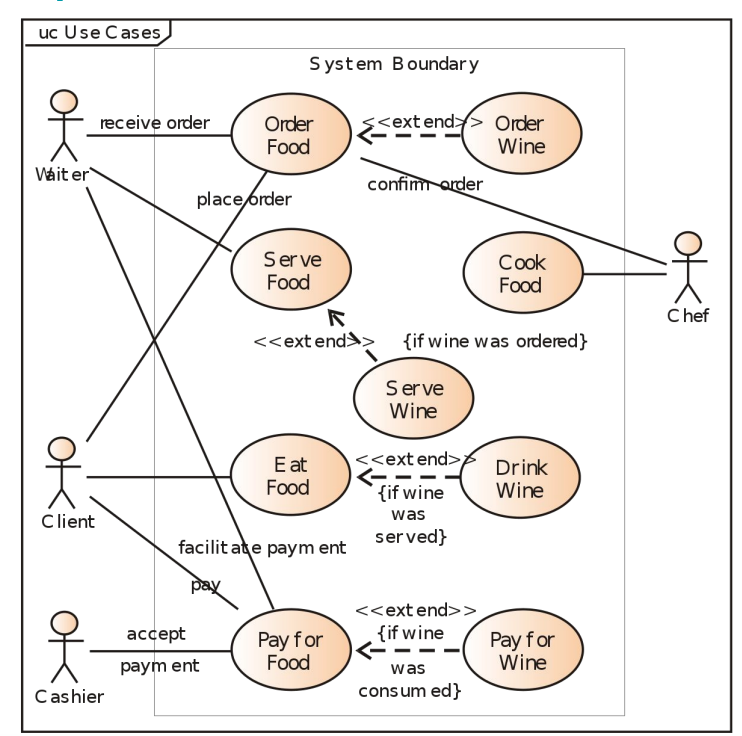
\includegraphics[angle=0, width=0.9\textwidth]{IMG/1} 
\end{figure}
\newpage

\subsection{Диаграмма классов}
\begin{figure}[!hbp]
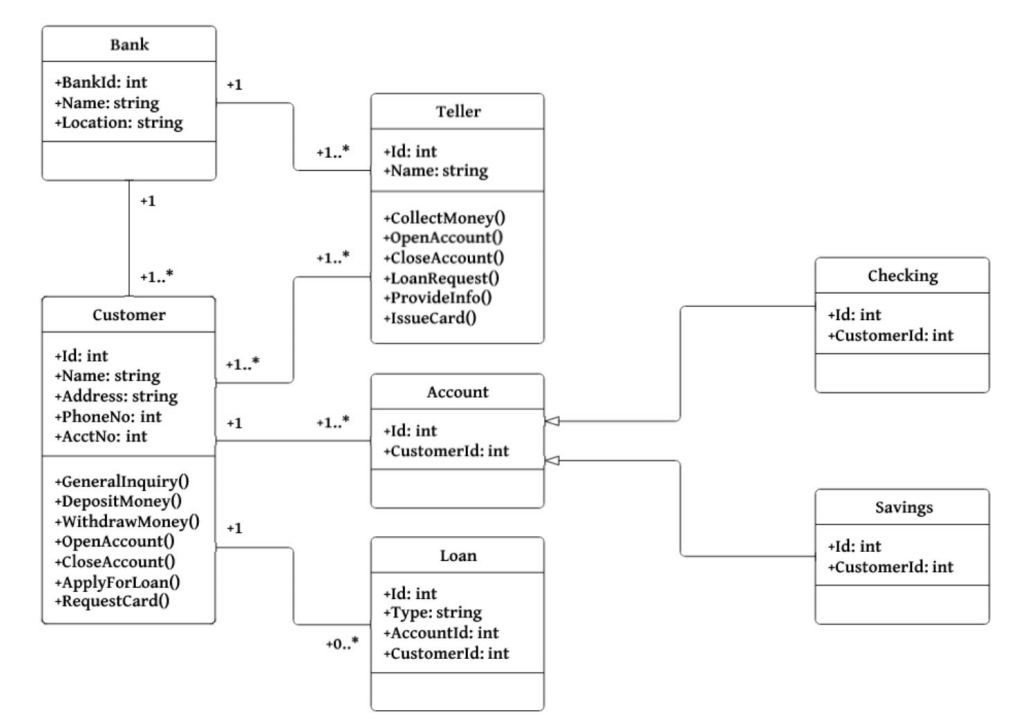
\includegraphics[angle=0, width=\textwidth]{IMG/2} \\
\end{figure}
Есть разные связи: 
\begin{enumerate}
\item[1] (Например король Артур и его лошадь) когда один объект так же перестает существовать
\item[1-1] Лошадь и всадник, когда они существуют по отдельности
\end{enumerate}
Так, например, в базе данных при удалении одного элемента, элементы, связанные с ним связью "1" так же будут не действительны.
\newpage

\subsection{Диаграмма последовательности}
\begin{figure}[!hbp]
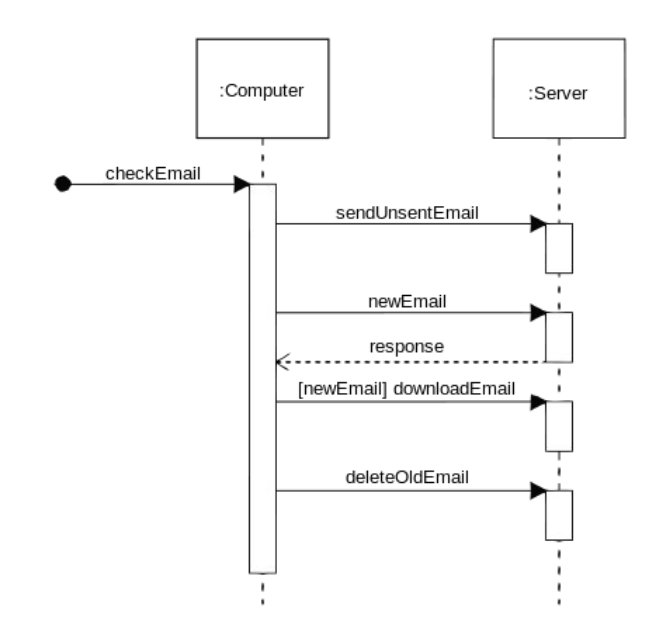
\includegraphics[angle=0, width=0.8\textwidth]{IMG/3} \\
\end{figure}
Рассмотрим на примере заселения.  В процессе участвуют Мы, Олег (поселяющий), Врач, кастелянша, деканат
Сначала мы идем к камендантше, затем идем к Олегу, он дает "a prove".  После идем к врачу, потом уже  к кастелянше.\\
Причем подключаются блоки в разных случаях: Сказал ли Олег Да или Нет? (Блок договориться с Олегом)\\
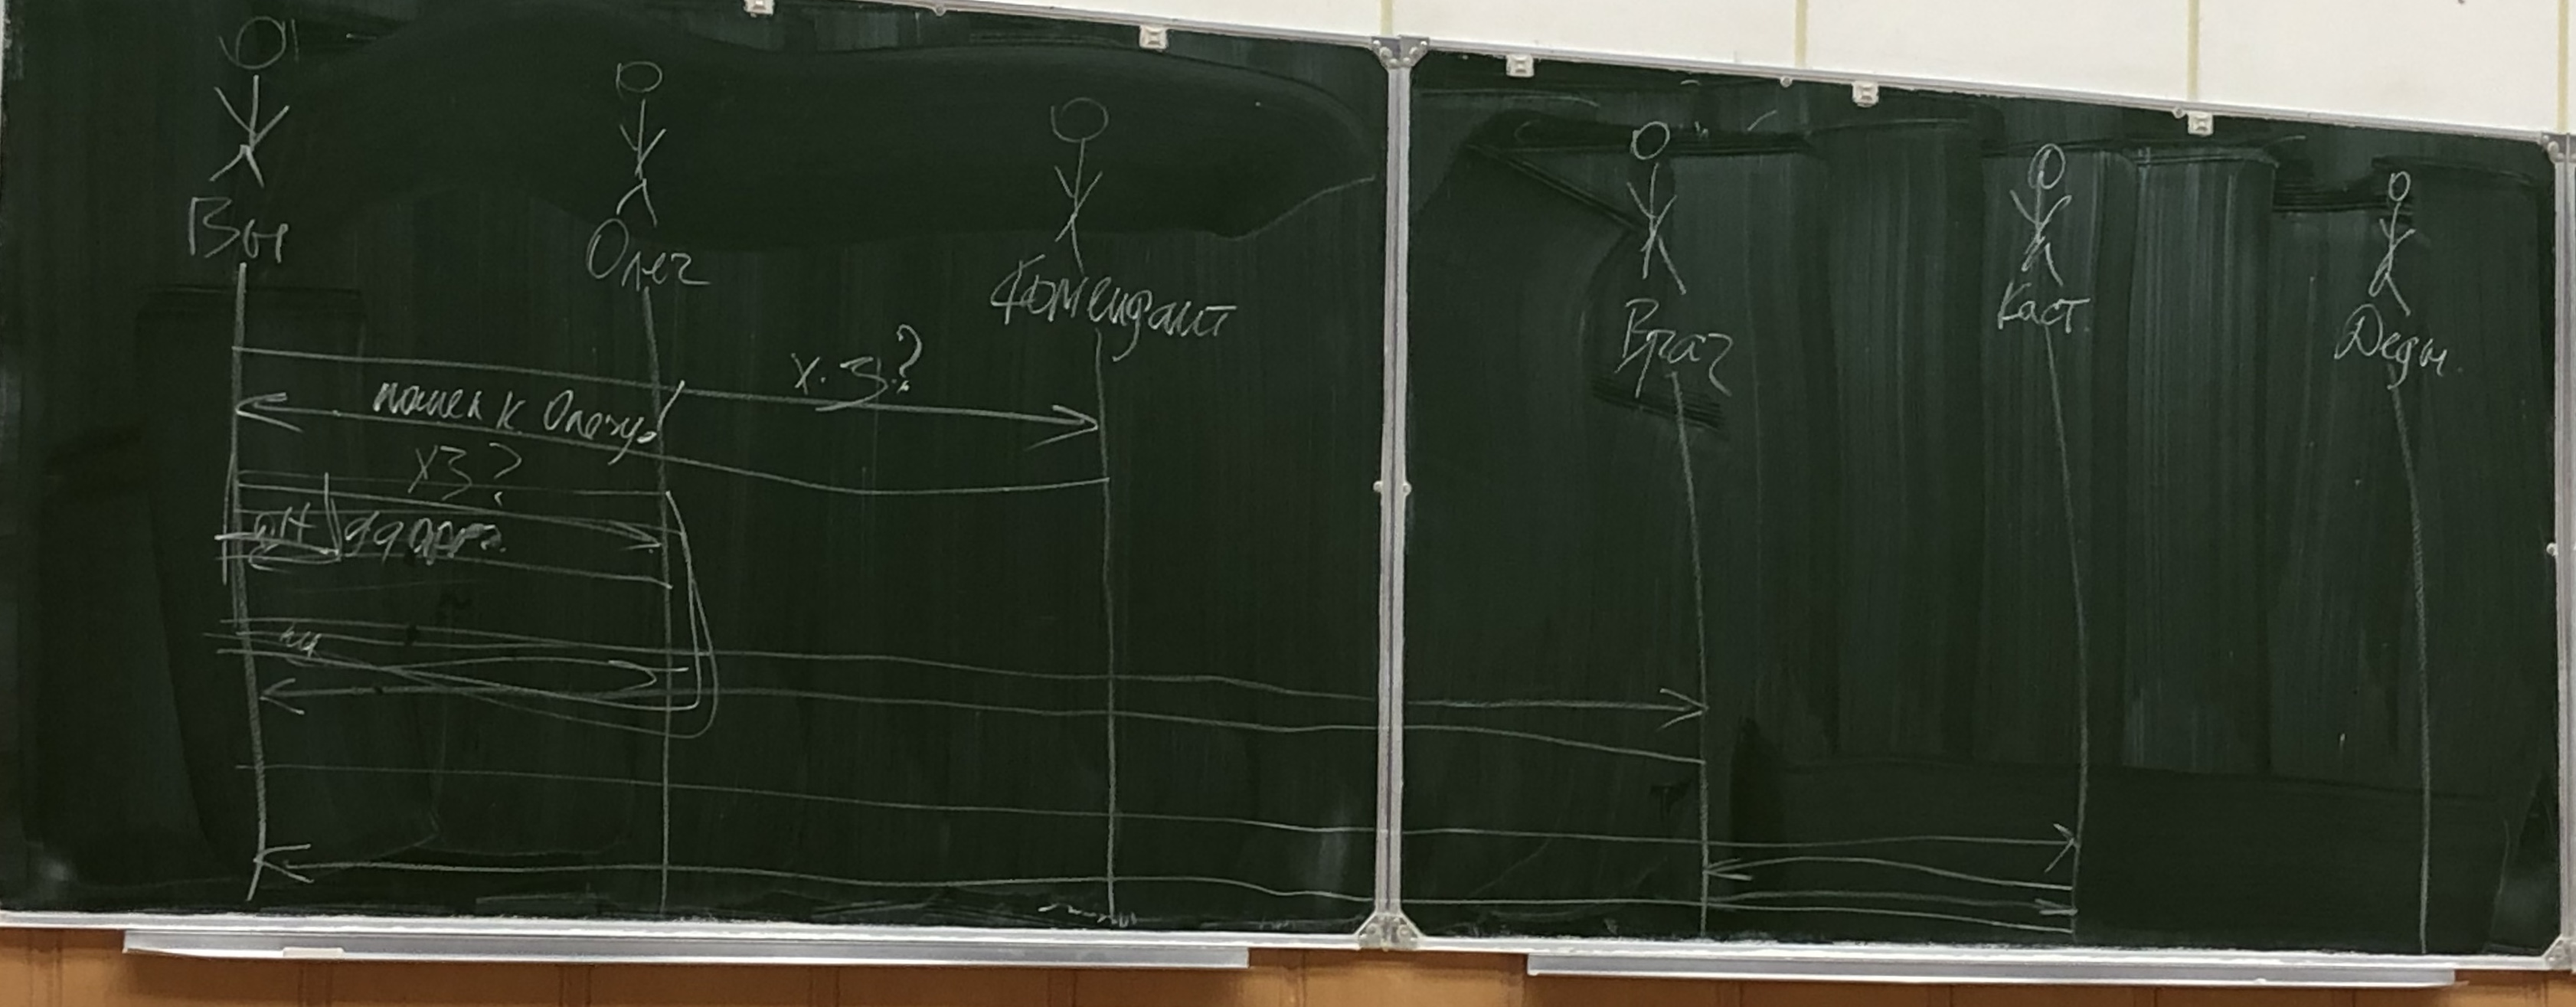
\includegraphics[angle=0, width=\textwidth]{IMG/IMG_0818.jpg} \\
\newpage

\subsection{Диаграмма состояний}
\begin{figure}[!htbp]
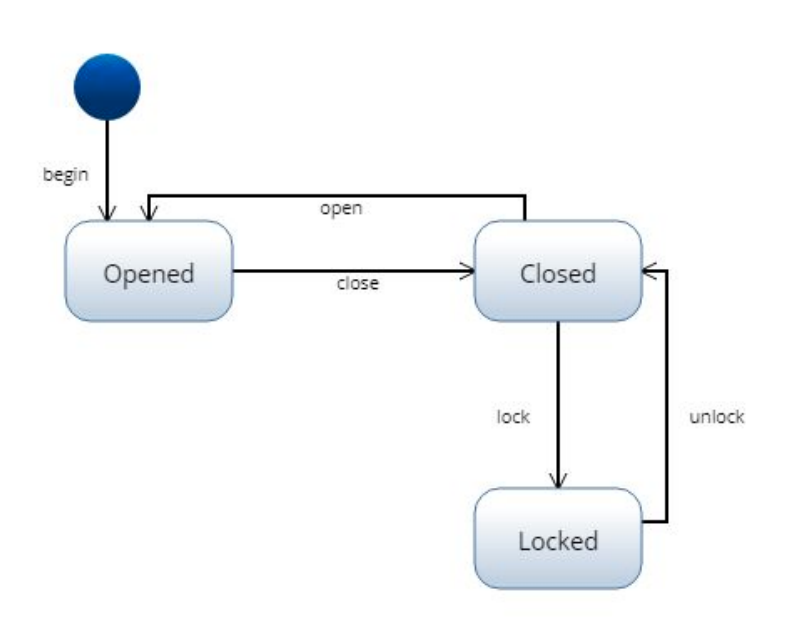
\includegraphics[angle=0, width=0.7\textwidth]{IMG/4} \\
\end{figure}
\begin{figure}[!htbp]
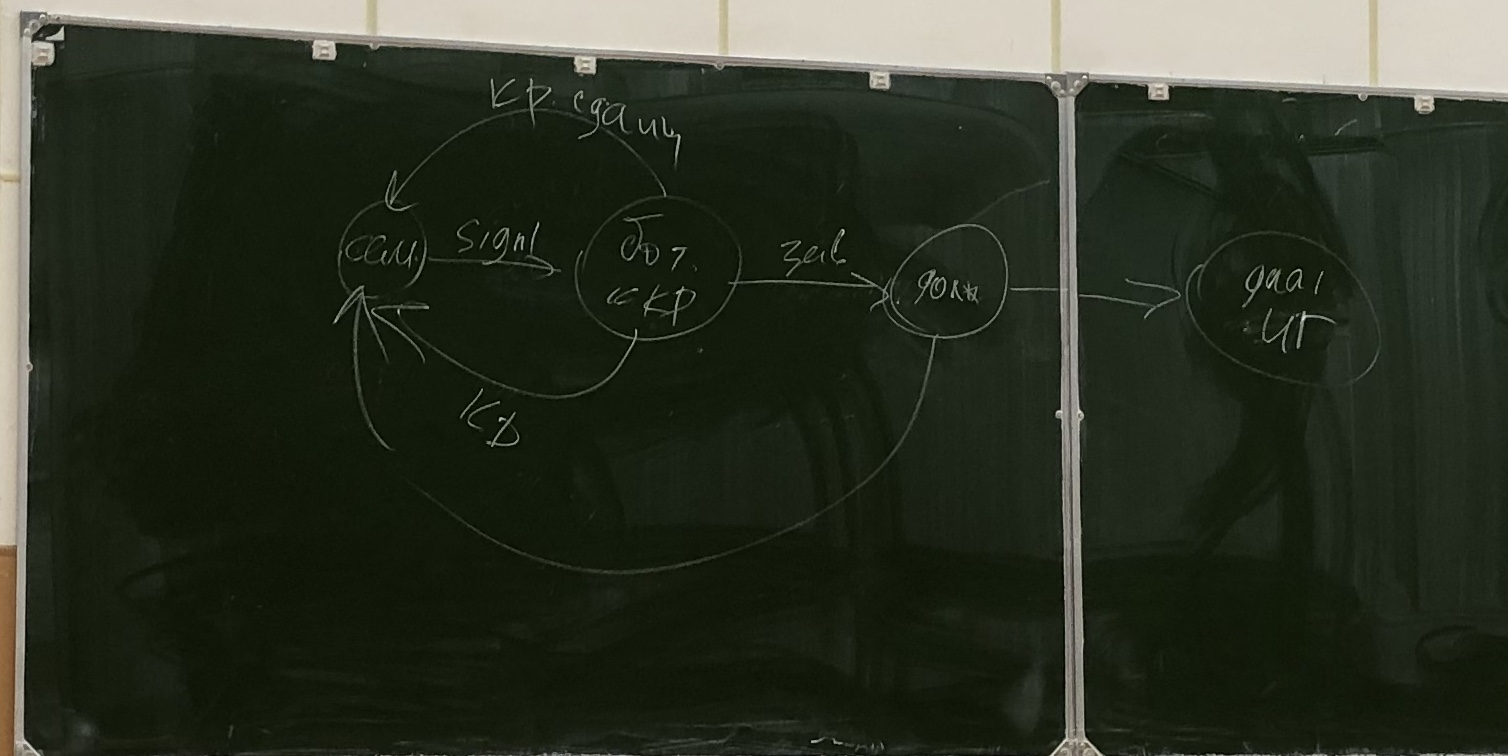
\includegraphics[angle=0, width=\textwidth]{IMG/IMG_0820.jpg} \\
\end{figure}
Диаграмма для студента:
Студент находится в состоянии "учусь", иногда переходит к состоянию "ботаю кр", дальше если кр не сдана то к состоянию "должник" и так далее...\\

Так с экраном. Если вы нажимаете Esc проваливаетесь на рабочий стол, дальше если открываете приложение проваливаетесь еще куда-то и т. д. \\
Еще когда мы открываем на телефоне карточки для платежа, яркость телефона выкручивается на максимум. Иногда телефон забывает вернуть яркость обратно, И ОН ВЫЖИГАЕТ ГЛАЗА) И нужно прописывать при переходе это.

\newpage
\subsection{Диаграма деятельности}
\begin{figure}[!htbp]
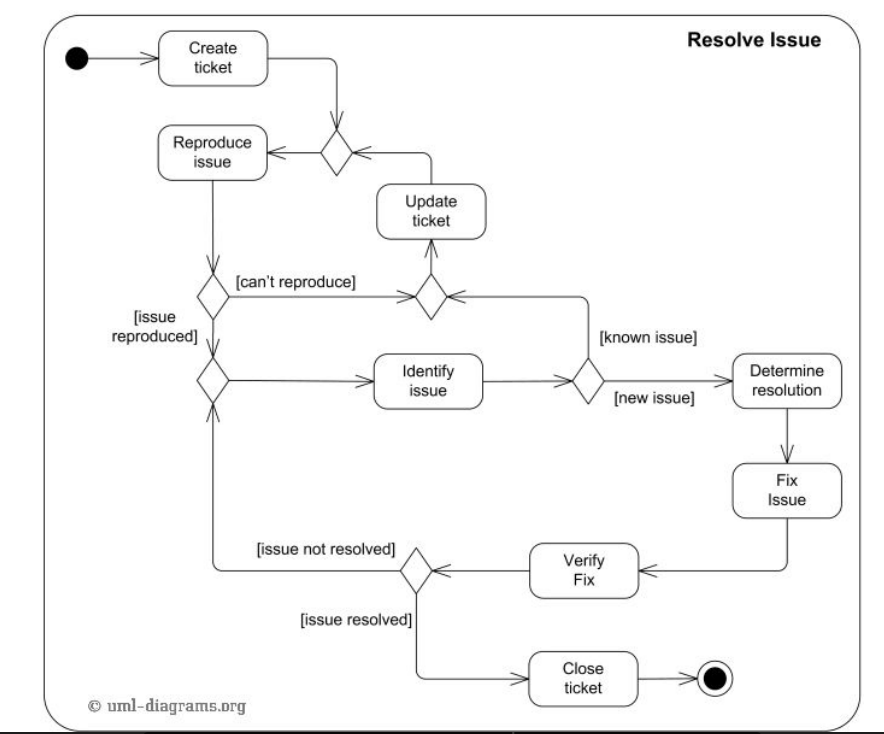
\includegraphics[angle=0, width=\textwidth]{IMG/5} \\
\end{figure}

Описание порядка набора действий на формальном языке с указанием что кто вызывает, по которой можно все восстановить. \\
\begin{figure}[!htbp]
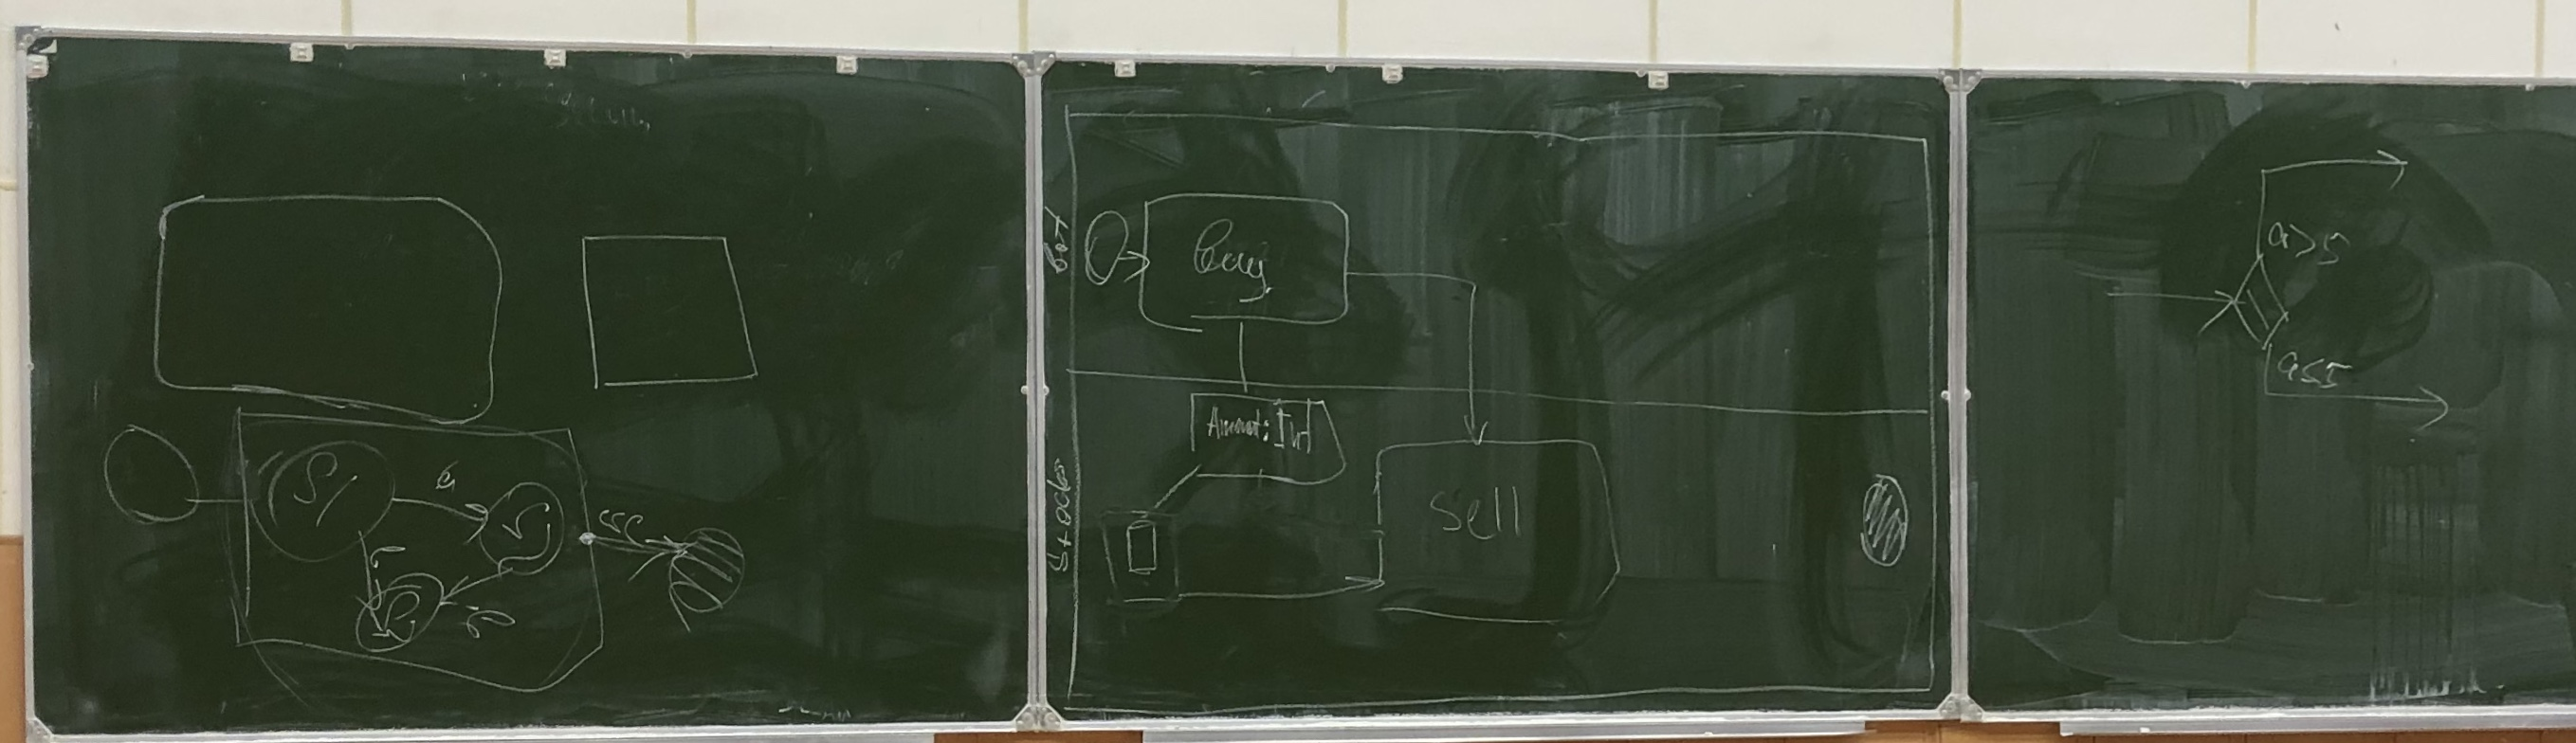
\includegraphics[angle=0, width=\textwidth]{IMG/IMG_0823.jpg} \\
\end{figure}

\#операция - с закругленными, объект - прямоугольник с острыми углами \\
например у bot 'а операция buy передает объект "ammount int" в операцию биржи(snoks) выполняя ее\\
\#терминальное состояние -- состояние конца операции для которой рисуется диаграмма \\
Еще есть условия (Например Ammount > 5/ <5...) \\
\#условия рисуются ромбиком\\\

\begin{figure}[!htbp]
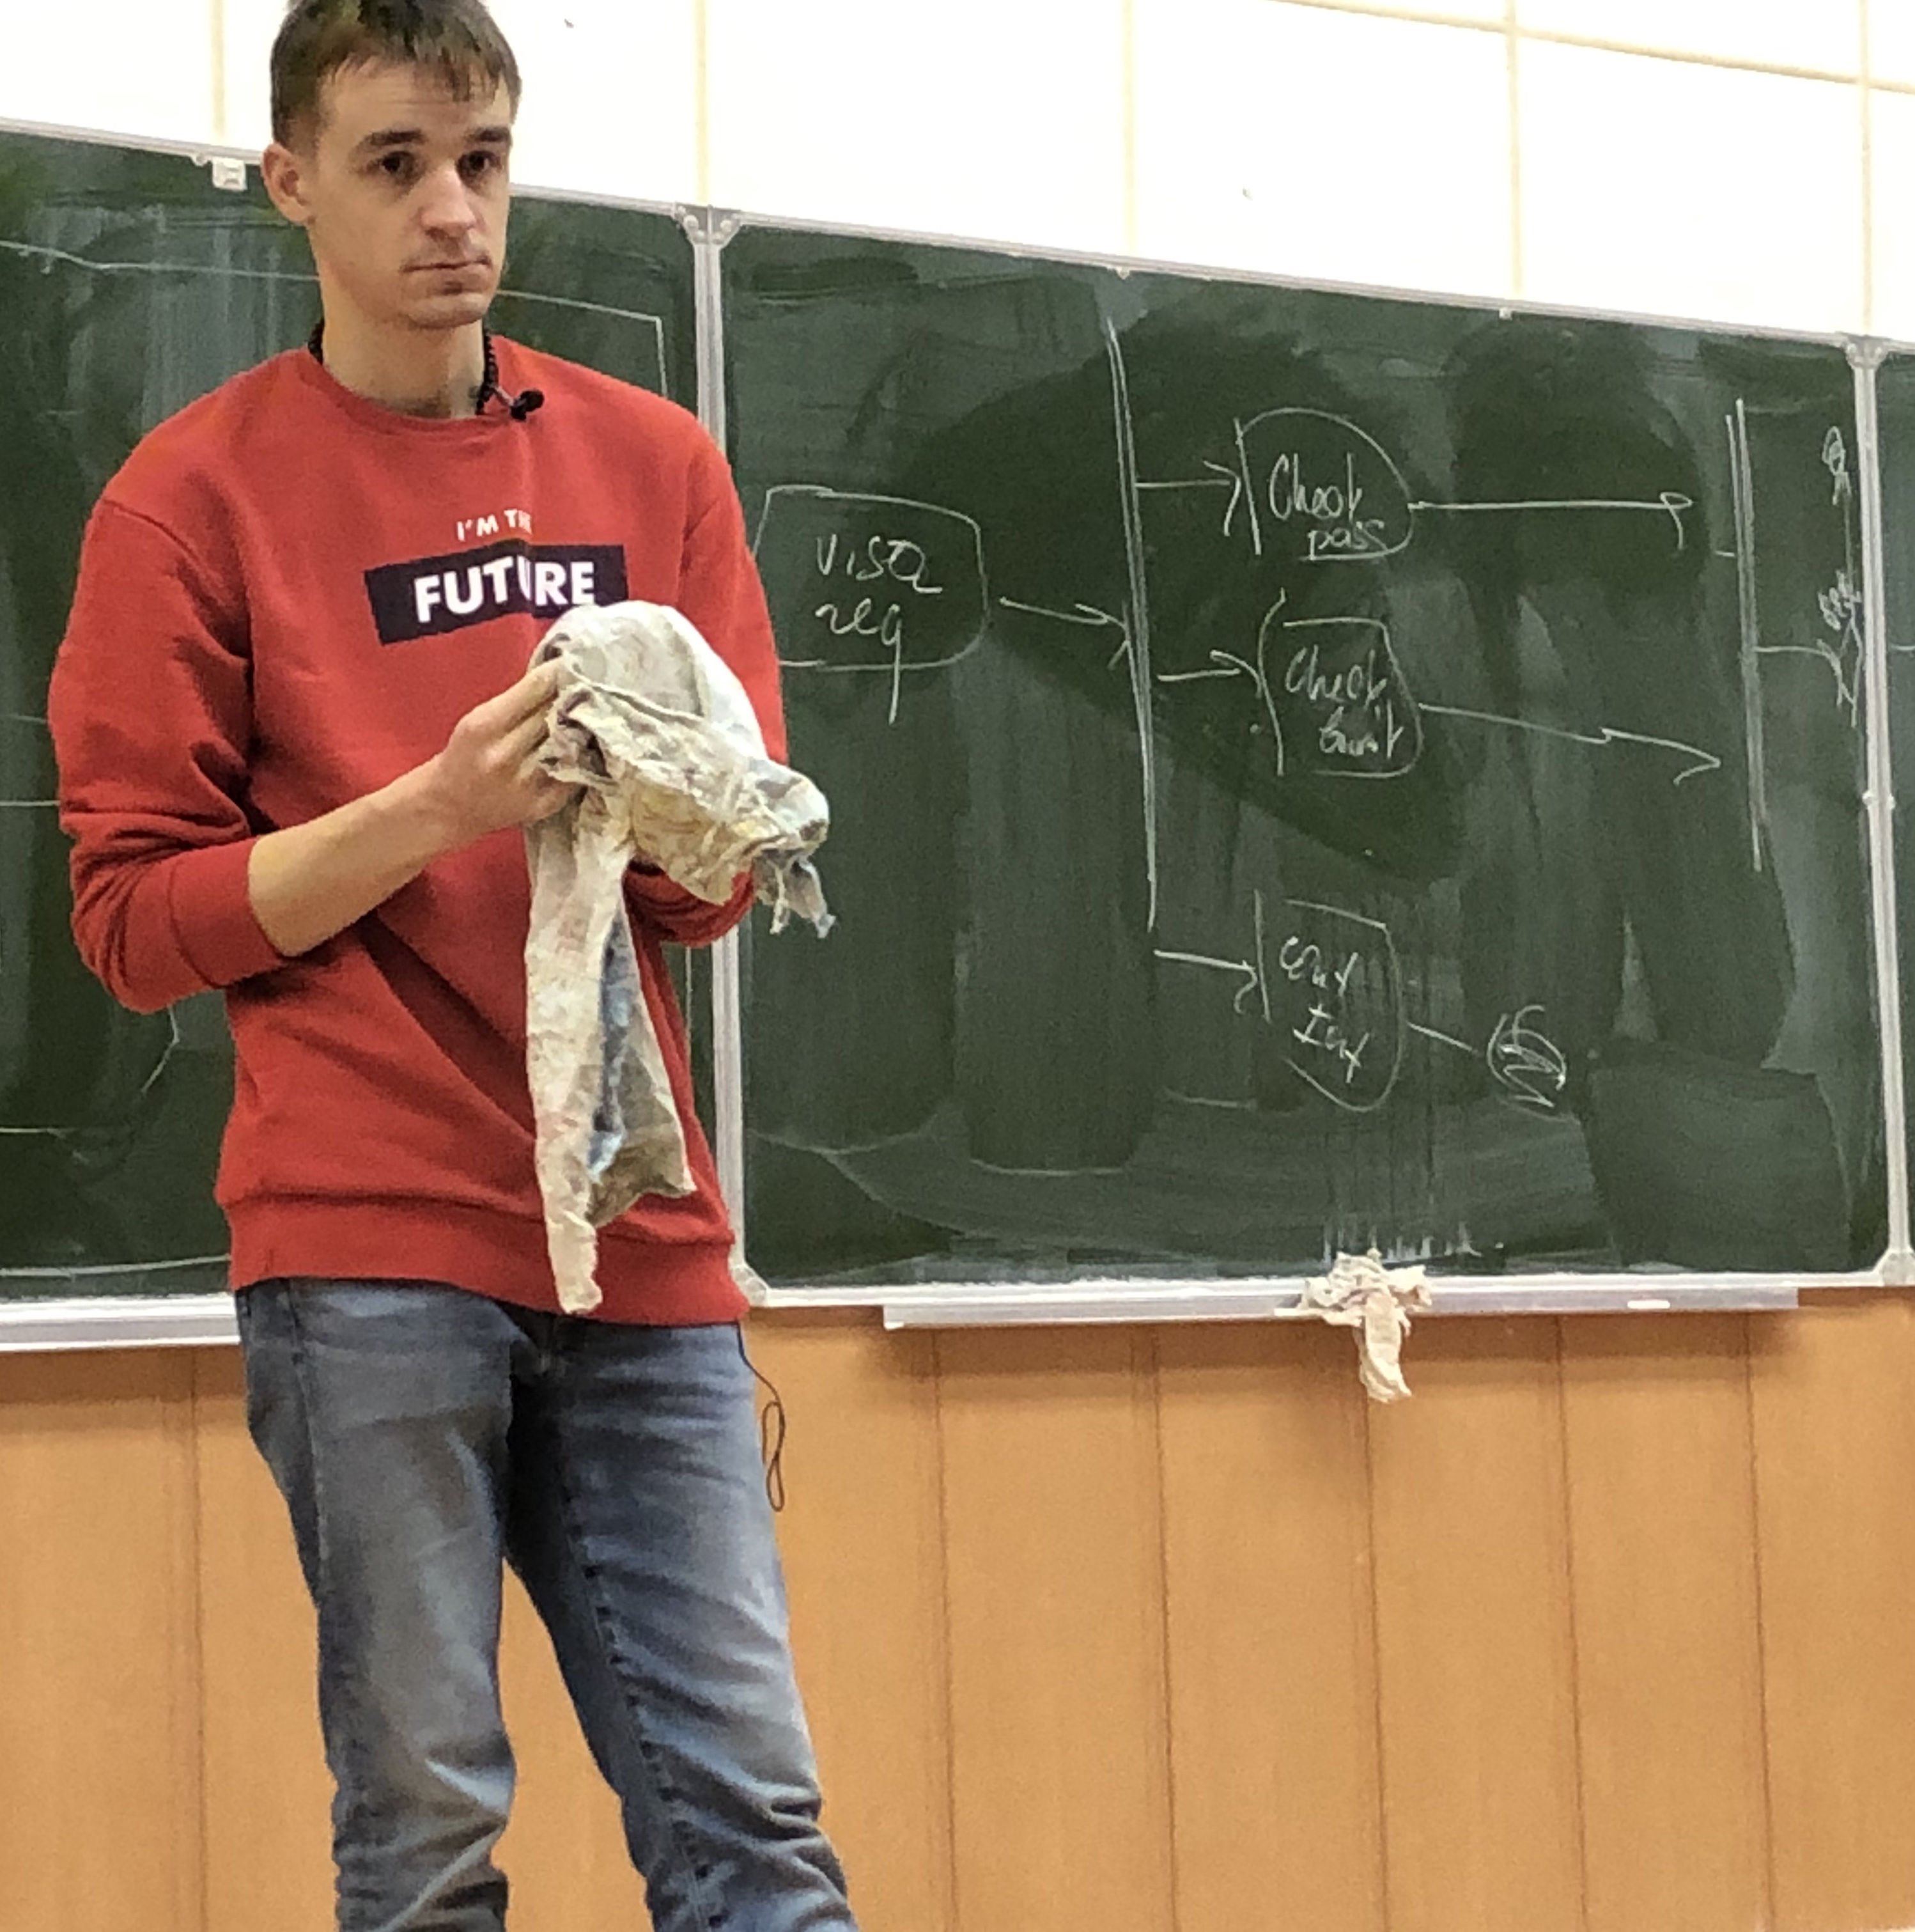
\includegraphics[angle=0, width=\textwidth]{IMG/IMG_0826.jpg} \\
\end{figure}

Еще есть распаралеливание и при завершении одного потока завершается только один поток. Потоки можно сливать. 
Например я хочу получить визу. Система паралельнор проверяет паспорт, проверяет банковский счет, и последняя, сразу завершаемая: передать в интерпол что поступил запрос. Дальше все сливается и виза дается/или нет.\\



\newpage
\section{Методологии разроботки (3я часть,  6я лекция)}
\begin{figure}[!htbp]

\includegraphics[angle=0, width=\textwidth]{IMG/10} \\
\end{figure}

\textbf{Выбор зависит от многих факторов:}
\b{enumerate}
\item Специфика проекта
    \b{itemize}
    \it Задача\\
    {\normalsize то есть что вообще в проекте делается}
    \it Область
    \it Требования\\
    {\normalsize что именно нужно достичь, как это должно работать и развиваться. Так же стоит разбить проект на этапы если требования слишком жесткие и трудные, достаточно самонадеянно думать что можно достичь требуемой производительности сразу.}
    \it Клиенты
    \it Заказчик\\
    {\normalsize Клиент и Заказчик предьявляюьт сроки, и нужно планировать разработку так чтобы эти требования удовлетворить}
    \e{itemize}
\it Система финансирования\\
{\normalsize Нужно платить сотрудникам, и если заказчик платит по достижению некоторых этапов разработки софта, то стоит делать поэтапную разработку. А если платят в конце, то может этапы и не нужны.}
\it Варианты поставки.\\
{\normalsize Нужно продумать как будет происходить внедрение обновлений. Например в одном случае проект требует того чтобы ты каждую неделю ездил к заказчику
домой, что не очень реально. А в другом, если например проект -- веб сайт, то его можно обновлять 
хоть каждый день}\\
\it \ldots\\ 
{\normalsize еще иногда приходится мириться с желаниями таких людей как team leader}
 \e{enumerate}
Нужно понимать что к проекту могут подходить разные методологии.

Теперь рассмотрим конкретные примеры методологий

\newpage
\subs{Модель водопада}
\begin{figure}[!htbp]
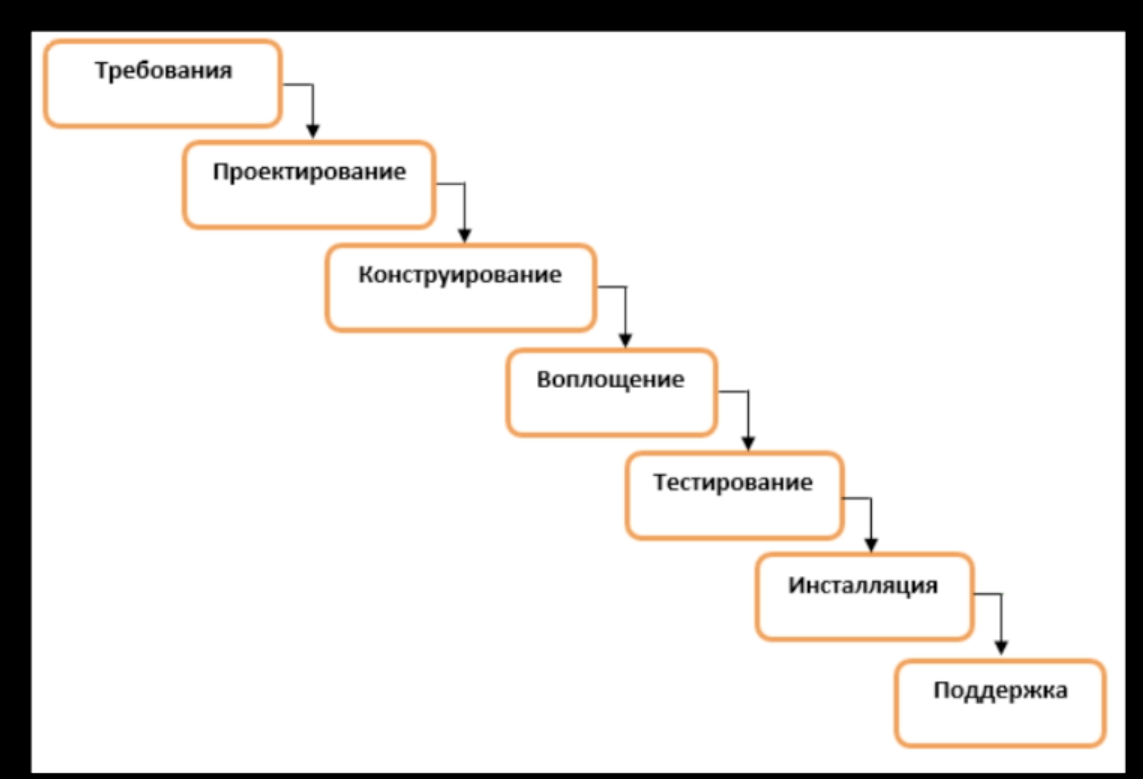
\includegraphics[angle=0, width=\textwidth]{IMG/11} \\
\end{figure}

\b{itemize}
\it она же Каскадная модель
\e{itemize}

Ее идея в том что:
\b{itemize}
\it Все стадии идут точно друг за другом
\it Следующая стадия не начинается пока не законченна предыдущая
\e{itemize}
Поэтому если сроки сдвигаются у одного этапа, они сдвигаются у всего проекта.\\
Плюсы методологии:
\b{itemize}
\it Четкие сроки
\it Четкая стоимость
\it Четкий результат
\e{itemize}

Но есть и минусы: \\
На момент когда проэкт будет готов супер развивающаяся технология может супер сильно развиться. И завод, строящийся с нуля уже устареет. Это проблема больших и долгих проектов. Для коротких проектов рассчитанных на 2-3 месяца эта модель уже хорошо подходит.


\newpage
\subs{V -- модель}
\begin{figure}[!htbp]
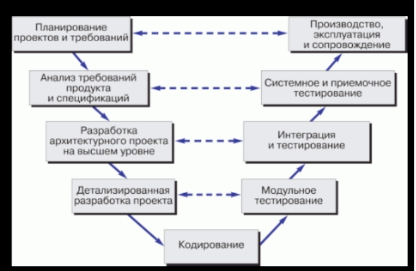
\includegraphics[angle=0, width=\textwidth]{IMG/12} \\
\end{figure}

\b{enumerate}
\it Верификация:
\b{itemize}
\it Требования бизнеса / 1. Конуепция
\it Функциональные требования /2. Высокоуровневая архитектура
\it Архитектура / 3. Детальные требования
\it Реализация
\e{itemize}
\it Валидация
\b{itemize}
\it Приемо-сдаточное тестирование /1. Поставка и проверка
\it Функциональное тестирование / 2. Приемо-сдаточное тестирование
\it Интеграционное тестирование
\it Модельное тестирование\\
{\normalsize то есть востребовано ли вообще то что мы сделали}
\e{itemize}
\e{enumerate}
V модель про жизнь проекта от высокоуровневых задач до низкоуровневых и назад к высокоурвневым. И также про горизонтальную связб между этапами.


\newpage
\subs{Инкрементная модель}
\begin{figure}[!htbp]
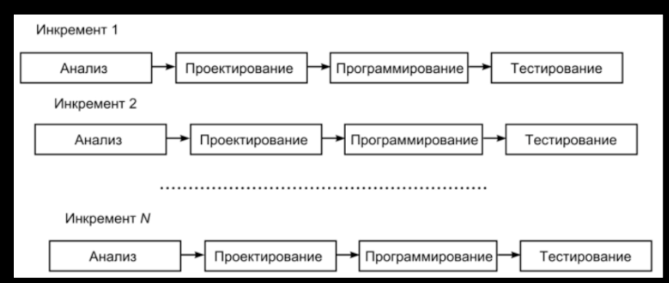
\includegraphics[angle=0, width=\textwidth]{IMG/13} \\
\end{figure}

\b{itemize}
\it Первая версия: базовая функциональность
\it Далее добавляются доп возможности
\it На каждом этапе производится:
    \b{enumerate}
    \it Определени требований
    \it Проектирование
    \it Кодирование   
    \it Внедрение
    \it Тестирование
    \e{enumerate}
\e{itemize}
Заранее знаем чем будем заниматься, то есть как будем улучшать.\\
\b{exmpl}
    Чатик, в котором улучшается количество поддерживаемых человек.
\e{exmpl}

\newpage
\subs{Итерационная модель}
\begin{figure}[!htbp]
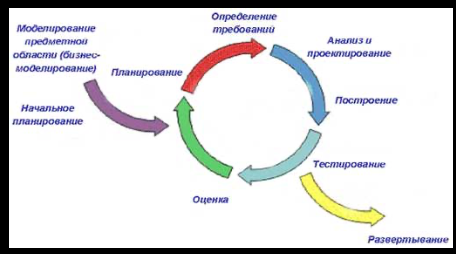
\includegraphics[angle=0, width=\textwidth]{IMG/14} \\
\end{figure}

\b{itemize}
\it Каждый этап - база для определения дальнейших требований
\it Важный момент - каждая новая версия полностью работоспособна
\it Требования к следующей версии составляются на основе анализа работа предыдущей версии
\e{itemize}
Эта модель в отличие от инкримеционной более гибка. Мы сразу не знаем всю картину шагов, каждый шаг продумывается на основе предыдущего шага.  \\
\b{exmpl}
    Чатик, в котором улучшения происходят на основе рякциии пользователей.\\
\e{exmpl}
В реальных проектах может происходить совмещение инкремеционной и итерационной моделей. Например Инкриментционная на старте, а потом итерационная.


\newpage
\subs{Спиральная модель}
\begin{figure}[!htbp]
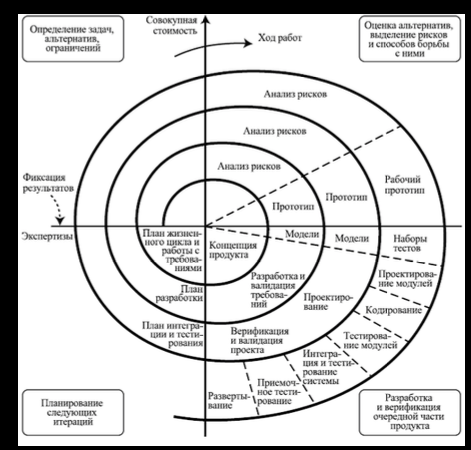
\includegraphics[angle=0, width=\textwidth]{IMG/15} \\
\end{figure}

\b{itemize}
\it Этапы:
    \b{enumerate}
    \it Планирование
    \it Анализ рисков
    \it Конструирование
    \it Оценка результатов
    \e{enumerate}
\e{itemize}

В спиральной модели все теже этапы: планирование, проектирование, ... . Эту модель выделяет то что в середине добавляется анализ рисков. \\
Применяется для сложных проектов в которые не понятно взлетят или нет. Проект дробится на этапы, и после каждого этапа идет анализ стоит ли докручивать софт. \
\b{exmpl}
    Приложение с тремя фильтрами. Оно работает и приносит деньги, и его можно улучшить добавив еще один фильтр. И далее анализируется нужно ли это или лучше направить силы на новый софт. 
\end{exmpl}

Как выбрать между Инкриментной, Итерационной и Спиральной моделями?
\b{enumerate}
\it Инкременционная -- когда развитие не такое долгое, и понятно каким должен быть финальный результат
\it Итерационная  -- для долгоиграющих пректов
\it Спиральная -- для проектов развивающихся с нуля, и проектов которые могут быть дропными. Дропными в том смысле что проект уже нормально работает в таком режиме, и его развитие на определенном жтапе можно прекратить.
\e{enumerate}

\newpage
\subs{RAD-модель}
Rapid Application Development Model (Быстрая разработка приложений)

\b{itemize}
\it Различные модули разрабатываются различными командами
\it Жестко ограниченное время
\it Интеграция отдельных модулей в один
\it Использование инструментов автоматической сборки и генерации кода
\it Этапы:
    \b{enumerate}
    \it изнес-моделирование
    \it Анализ и создание модели данных
    \it Анализ и создание модели процесса
    \it Автоматическая сборка приложения
    \it Тестирование
    \e{enumerate}
\e{itemize}
В такой модели часто применяется автоматическая генерация кода (для связи между модулями?). Из-за этого страдает производительность.\\
Такую модель применяют к системам с большим количеством модулей и низкими требованиями к производительности. И также применяют для быстрой разработки приложений.\\
 Такая модель сейчас довольно популярна на рынке.
\b{exmpl}
    Приложение с тремя фильтрами. Оно работает и приносит деньги, и его можно улучшить добавив еще один фильтр. И далее анализируется нужно ли это или лучше направить силы на новый софт. 
\end{exmpl}


\newpage
\subs{Agile}
Rapid Application Development Model (Быстрая разработка приложений)
\begin{figure}[!htbp]

\includegraphics[angle=0, width=\textwidth]{IMG/17} \\

\end{figure}
\b{itemize}
    \it Семейство гибких методологий разработки
    \it Короткие итерации
    \it Разные метрики качества работы \\
    {\ns Присваиваем текущим задачам величину работы и ставим целью сделать за неделю определенное количество работы}
    \it Много разных конкретных подходов
    \it Этапы:
        \b{enumerate}
        \it изнес-моделирование
        \it Анализ и создание модели данных
        \it Анализ и создание модели процесса
        \it Автоматическая сборка приложения
        \it Тестирование
        \e{enumerate}
\e{itemize}
Плюсы Agile то что благодаря тому что ставим целью выполнить определенный объем работы, можем быстро реагировать на изменения среды. Например доюавить в прилодение вохможность загружать картинки с недавно ставшего популярным приложения.\\
 Минусы:из-за такой гибкости сроки довольно размыты, и процесс может затягиваться.\\

\textbf{Agile-манифест}
\b{itemize}
    \it ЛЮДИ И ВЗАИМОДЕЙСТВИЕ важнее процессов и инструментов
    \it РАБОТАЮЩИЙ ПРОДУКТ важнее хорошей документации
    \it СОТРУДНИЧЕСТВО С ЗАКАЗЧИКОМ важнее условий контракта
    \it ГОТОВНОСТЬ К ИЗМЕНЕНИЯМ важнее первоначального плана
\e{itemize}

 \subs{Итоги}
 Выжно учесть что в одном проекте разные его части могут совмещать разные методологии. Например frontend быть основан на ajile, а backend  на итерированиях.\\
 И еще раз: при выборе методологии смотреть в начало, и отталкиваться от того что мы хотим в проекте: Сделать так чтобы всем нравилось, или точно сделаьть определенные вещи в определенный срок и тп

\newpage
\section{Continuous Integration (7я лекция)}
 Continuous Integration -- набор методик и практик выстраивания процесса.
\begin{figure}[!htbp]
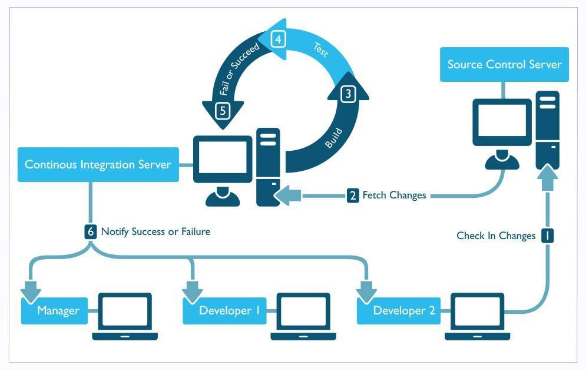
\includegraphics[angle=0, width=\textwidth]{IMG/16} \\
\end{figure}
Все это дело заключается в том, что девелоперы комитят изменения в какую-то систему контроля версий.
Далее после того как изменения запушены, сервер делает вывод что эти изменения нужно подключить к проекту. Хотя лучше сказать что Continous integration Server непрерывно следящий за сервером контроля версий замечает изменеия. И дальше принимает решение успешна или не успешна сборка. Неуспешна в двух случаях: Или сам проект не собрался, или какие-то тесты не пройденны.\\
Этот процесс может быть довольно накладным, если сборка очень долгая или разработчиков очень много. Поэтому в случаях больших проектов обычно устанавливают таймер сборки проекта, например, каждую ночь.
\begin{figure}[!htbp]
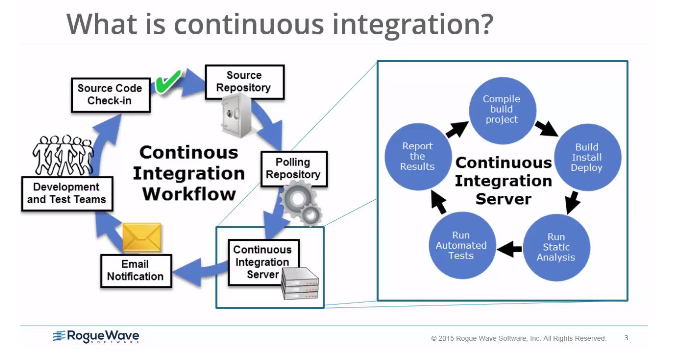
\includegraphics[angle=0, width=\textwidth]{IMG/18} \\
\caption{типичный цикл процесса contin int}
\end{figure}

\newpage
\begin{figure}[!htbp]
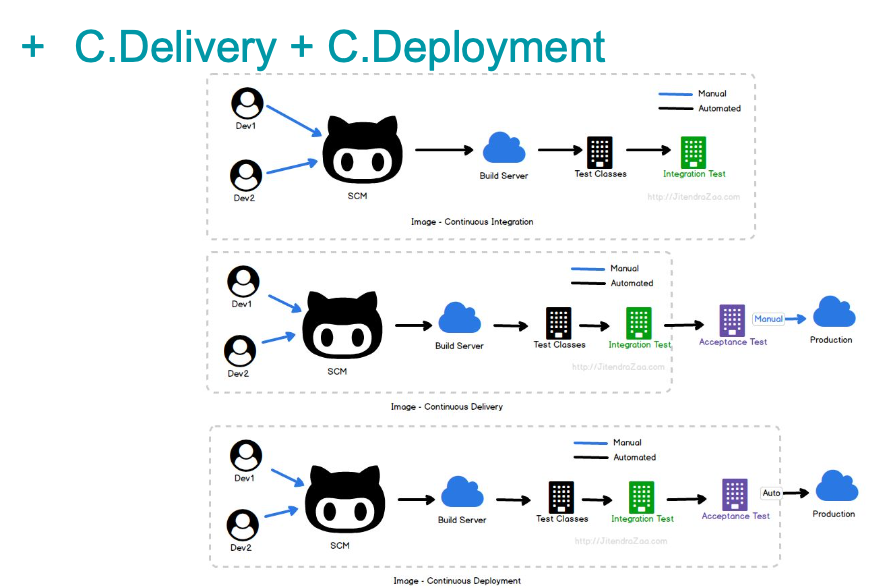
\includegraphics[angle=0, width=\textwidth]{IMG/19} \\
\caption{типичный цикл процесса contin int}
\end{figure}
Continuous Delivery - расширение понятия continuous ibtegration, в котором добавляется автоматическая финальная проверка. Но финальная проверка с добавлением обновления в продакшн остается за человеком\\
Continuous Deployment - то же что Continuous Delivery, но финальная проверка выполняется так же автоматически. Применяется на веб сайтах.


\newpage
\section{А как у нас?}
\subs{Этап проектирования}
\b{enumerate}
    \it Идея
    \it Первоначальное обсуждение
    \b{itemize}
        \it Что
        \it Зачем
       \it В какую версию\\
       {\normalsize Нужно понимание в какую версию обозначает сроки выполнения задачи. То есть обычно в проекте есть сроки релищов и данная задача может занимать гораздо больше времени чем оставшеесе время до следующего релиза}
        \it Как именно будет реализовано
    \e{itemize}   
    \it Несколько итераций обсуждений проектного документа\\
       {\normalsize Обсуждение задачи с другими командами, которые потребуются для реализации данной задачи. Этот процесс выглядит так: вы пишете проектный ддокумент и рассылаете его заинтерисованным лицам, и далее после обсуждений в проект вносятся изменения. Далее этот проект уже идет к лидеру и он одобряет/не одобряет / корректирует}
    \it Финальное согласование
\e{enumerate}

\newpage
\subs{Этап реализации}
\b{enumerate}
    \it Отдельная ветка в SVN для задачи\\
       {\normalsize Тут есть вопрос от чего нужно делать fork для нашей ветки. Самое простое это делать форк от последнего релиза. Но  это может вызвать проблемы если последний релиз был слишком давно. Брать последнюю версию же черевато ошибками. Решение -- регулярно далать сборки (например каждые день)  и держать и обновлять свужую last sucsessfull версию, то есть версию котораю была при последней успешной сборки. И уже от нее игать.}
    \it Реализация и отладка локально
    \it Локальное тестирование\\
       {\normalsize Тут проверяется что то что было созданно работает ровно так было принятно в финальной версии проекта.}
    \it Поднятие версии\\
    {\ns На этом этапе везде в этапе где указана версия она меняется на новое число.}
    \it Интеграционная сборка на системе CI (в ручном режиме)\\
       {\normalsize Тут проводится ограниченное тестирование, вместо полного. Это делается поскольку полное тестирование может занимать 5-6 часов, что слишком долго.}
    \it Если надо - повторить п.2-5
    \it Интеграционная сборка с полными тестами
\e{enumerate}

\newpage
\subs{Этап сдачи задачи}
\b{enumerate}
    \it Код-ревью
    \it Исправить имеющиеся замечания, вернуться в п.1
    \it Подготовка документации по задаче \\
       {\normalsize Тут пишется коротенькая черновая документация, которая потом будет использованна уже для нормальной пользовательской документации.}
    \it Отправка задачи на независимую проверку (сборка + документация)\\
       {\normalsize Например, проверять может другая команда. Для проверки проверяющие получают документацию и готовое улучшение, и составляет критические замечания, как со стороны пользователя. Код и технический проект на этом этапе не смотрятся.}
    \it Исправить имеющиеся замечания, вернуться в п.4
    \it Финальный “ОК” на в
   литие задачи в ствол у отв.
    \it Влить в ствол
    \it Закрыть задачу
\e{enumerate}

\newpage
\subs{Подготовка к выпуску версии}
\b{enumerate}
    \it Введение моратория на разработку\\
       {\normalsize Мараторий это дедлайн срокоа до которого можно отправлять задачи на вливание к подготавливаемой новой версии. Если программисты не успели, их задача перенаправляется на следующую версию.}
    \it Проверка “висящих” задач
    \it Влитие оставшихся задач 
    \it Введение моратория на изменения в ствол (только искл.случаи)
    \it Сборка кандидата в релиз\\
       {\normalsize Тут отлавливают в основном интеграционные ошибки несовместимости подготовленных задач.}
    \it Тестирование (автоматическое и ручное)\\
       {\normalsize Если очередная задача была сочтена недостаточно хорошей. Например, из за производительности, то задача исключается из ствола и переводится на следующий релиз.}
    \it Исправление ошибок, возвращаемся в п.6
    \it Релиз кандидата
\e{enumerate}


\newpage
\section{Структурные и поведенческих паттернов}

\subs{Структурные }
\subs{Bridge}
Отделить две сущности от друга для дальнейшей реализации\\
\b{exmpl}
Есть какой-то объект (контроллер с разными функциями: кнопка, список) который нужно немного по разному реализовывать на виндоусе и линуксе. И вместо разных реализаций каждого объекта контрола, можно реализовать паттерн OS который будет иметь разные методы(виндоус, линукс) который будет приспосабливать методы контрола под определенную ОС.\\
В данном примере контрол абстракция, а OS - реализация.\\
Другие примеры\\
	\b{itemize}
		\it Производство (общение) пультов и телевизоров
		\it Графические редакторы (фигуры и заливки)
	\e{itemize}
\e{exmpl}
\b{exmpl}
    Приложение с тремя фильтрами. Оно работает и приносит деньги, и его можно улучшить добавив еще один фильтр. И далее анализируется нужно ли это или лучше направить силы на новый софт. 
\end{exmpl}



\end{document}


\subsection{}
\begin{enumerate}
\item 
\item 
\item 
\item 
\item 
\item 
\item \end{enumerate}
\textbf{} %make bold
\hangindent=6cm \hangafter=2 \noindent % 1st - indent length, 2nd - numb of str without indent

\definecolor{linkcolor}{HTML}{799B03} % цвет ссылок
\definecolor{urlcolor}{HTML}{799B03} % цвет гиперссылок
 
\hypersetup{linkcolor=linkcolor,urlcolor=urlcolor, colorlinks=true}

%%%%%%%%%%%%%%%%%%%%%%
Редакторы:  \href{https://vk.com/akira33333}{Фреик Александр} \href{https://github.com/Falier77777}{git}\\

\begin{titlepage}
\begin{center}
\large\textbf{Московский Физико-Технический Институт}\\
\large\textbf{(государственный университет)}
\vfill
\line(1,0){350}\\[2mm]
\huge\textbf{Технологии программирования\\ 2 семестр, 2020 год}\\
\line(1,0){350}\\[2mm]
\vfill
\line(1,0){350}\\[1mm]
{\normalsize Лектор: Старичков Никита\\\
Редакторы:  \href{https://vk.com/akira33333}{Фреик Александр} \href{https://github.com/Falier77777}{git}}\\
\large ФПМИ\\
\line(1,0){350}\\[1mm]
\end{center}
\end{titlepage}
%%%%%%%%%%%%%%%%%%%%%%%
